\section{Siamese Multi-Object Tracking and ReID}
\label{sec:SiamMOTandReID}

% ##############################################################################
\subsection{Motivation}

The use of \gls{reid} has been emphasized numerous times during our preliminary research. We conjectured that once full occlusion ensues, the \gls{reid} mechanism could be adopted to recover the lost track. The presence of occlusion percolates traffic scenes, especially if the camera does not view the road from a higher position. At the beginning of our research, we worked on the \interreg{} project in which we tackled vehicle tracking when the camera was positioned next to the road (\figtext{}~\ref{fig:InterregDatasetSample}). Such a setup inexorably led to situations in which a vehicle appeared for a second on the left side of the frame, then ended up fully covered by a truck, and re-appeared for a minuscule amount of time at the other side of the frame, making the occlusion inevitable. The task of maintaining the same object identifier was often impossible with a high degree of precision.

% ##############################################################################
\subsection{Proposed ReID-Enhanced Architecture}
\label{ssec:ProposedReIDEnhancedArchitecture}

We adopted the object \gls{reid} approach published in~\cite{luo2019bagoftricksreid}, a simple yet very robust framework for person \gls{reid}. We employed this architecture (\figtext{}~\ref{fig:BagOfTricksReIDArchitecture}) for vehicle \gls{reid} due to its simplicity accompanied with \gls{sota} performance at the time of publishing.

% ------------------------------------------------------------------------------
\begin{figure}[!t]
    \centering
    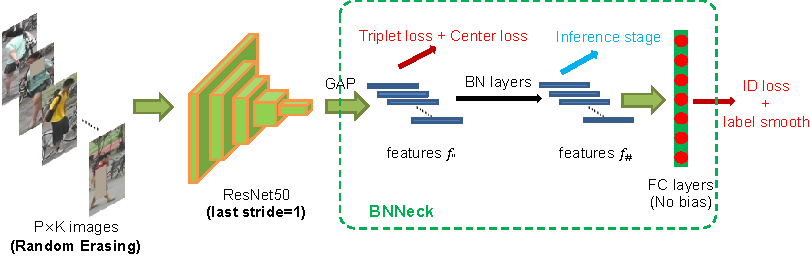
\includegraphics[width=\linewidth]{figures/siamese_tracking/bagoftricks_reid_architecture.pdf}
    \caption[\gls{reid} baseline]{A object \gls{reid} baseline which we used for our experiments. \externalsrc{\cite{luo2019bagoftricksreid}}}
    \label{fig:BagOfTricksReIDArchitecture}
\end{figure}
% ------------------------------------------------------------------------------

% ##############################################################################
\subsection{Training Phase}

Since this experiment was the first one we embarked upon, we tried to avoid modifications to the underlying model. Only upon obtaining prospective improvements would we consider incorporating the object \gls{reid} into the whole pipeline. We employed an external object \gls{reid} network to perform embedding computation during the inference. As for the training of the \gls{reid} network, we adopted a standard approach of using the triplet loss (\eqtext{}~\ref{eq:TripletLoss} on page \pageref{eq:TripletLoss}) in conjunction with the categorical cross-entropy loss. We trained the model using the \verisss{} dataset (\sectiontext{}~\ref{ssec:DatasetVeRI776} on page \pageref{ssec:DatasetVeRI776}) on which the evaluation was performed, too. The model was trained to produce $l_2$-normalized embedding vectors that were then used to measure the degree of similarity between vehicles.

% ##############################################################################
\subsection{Inference Phase}

The online solver algorithm was the primary suspect for potential improvements due to its inherent simplicity compared to the rest of the architecture. The aim was to adopt the already trained \gls{reid} model to help re-instantiate lost tracks due to occlusion. This external module would be invoked on-demand as part of the online solver phase. At this stage of research, we did strive for simplicity rather than efficiency. Consequently, the model inference was substantially impaired by a four-fold speed reduction.

We isolated the modifications to the inference phase only to the online solver itself. Thus, we developed a whole new algorithm that handled the newly trained external model, too. The original processing steps of the online solver are outlined in \figtext{}~\ref{fig:SiamMOTOnlineSolver}. Our custom inference algorithm is described \algtext{}~\ref{alg:OnlineSolverReID}.

The algorithm works as follows. The input to the online solver is the set of active tracks, dormant tracks, and newly detected (still unassigned) objects. As in the original implementation, the greatest emphasis during the \gls{nms} processing is put on the active tracks, then dormant tracks, and the last ones are the new detections. This ranking establishes the priority with which the \gls{nms} algorithm processes the inputs. Our approach was based on altering the first \gls{nms} phase by incorporating only the active tracks and unassigned detections (hence the name ``non-dormant'' in the pseudocode). Thus, if the overlap between an active track \gls{bbox} and detection was too high (above the value of $t_{nms}$), we considered them to be the same object, and thus the active track was preserved.

Having suspended the removed active tracks, we adopted Munkres' algorithm~\cite{munkres1957assignment} to solve the linear sum assignment optimization problem. It is reasonable to assume that a new detection can be assigned to only one dormant track and vice versa, if necessary. The cost matrix was computed based on the cosine similarity (\eqtext{}~\ref{eq:CosineSimilarity} on page \pageref{eq:CosineSimilarity}) between the embedding vectors belonging to the regions of the unassigned detections and the dormant tracks. However, only the visual features where the dormant object was last visible (its visibility confidence was above the threshold $t_{track}$) were used, as we assumed the object might have been fully occluded. The task was to find an optimal assignment between the new detections with sufficiently high confidence (above the threshold $t_{resume}$) and the dormant tracks. Upon obtaining the assignment matrix, we processed all possible pairs and if the similarity between the embedding vectors surpassed the value of $t_{sim}$, we then resumed the dormant track and re-used the new detection for the object \gls{bbox}.

Subsequently, we collected all the remaining unassigned detections the confidence of which was above $t_{start}$ and initiated new tracks based on them. At last, we searched for active tracks with low visibility confidence (below the threshold $t_{track}$) to suspend them, to make them dormant.

\begin{algorithm}[t]
    \caption[\gls{reid}-enhanced online solver inference]{\gls{reid}-enhanced online solver inference. This algorithm receives active ($\mset{A}$) and dormant ($\mset{D}$) tracks together with unassigned ($\mset{U}$) detections on the input. Besides, there are four threshold parameters, the \gls{nms} overlap ($t_{nms}$), and three confidence-related inputs, namely the minimum value for the track to stay active ($t_{track}$), the minimum value for the track to become resumed ($t_{resume}$), and the minimum value for the track to start from an unassigned detection ($t_{start}$). Usually, $t_{track} < t_{resume} < t_{start}$. In practice, these values may be $0.3$, $0.4$, and $0.5$, respectively.}
    \label{alg:OnlineSolverReID}
    \begin{algorithmic}[1]
        \Function{OnlineSolverReID}{$\mset{A}$, $\mset{D}$, $\mset{U}$, $t_{nms}$, $t_{track}$, $t_{resume}$, $t_{start}$, $t_{sim}$}

        \State $\mset{\bar{D}}$ $\gets$ \Call{merge}{$\mset{A}$, $\mset{U}$}
        \Comment{non-dormant items (active tracks, unassigned dets.)}

        \State $\mset{\bar{D}}_{nms}$ $\gets$ \Call{NMS}{$\mset{\bar{D}}$}
        \Comment{non-maximum suppression (\algtext{}~\ref{alg:NonMaximumSuppression} on page \pageref{alg:NonMaximumSuppression})}

        \State $\mset{A}_{nms}$, $\mset{U}_{nms}$ $\gets$ \Call{split}{$\mset{\bar{D}}_{nms}$}
        \Comment{``after-\gls{nms}'' active tracks and unassigned dets.}

        \State $\mset{R}$ $\gets$ \Call{get_removed}{$\mset{A}$, $\mset{A}_{nms}$}
        \Comment{obtain \gls{nms}-removed active tracks}

        \State \Call{suspend_tracks}{$\mset{R}$}
        \Comment{suspend \gls{nms}-removed active tracks}

        \State $\mset{U}_{resume}$ $\gets$ \Call{get_resume_dets}{$\mset{U}_{nms}$, $t_{resume}$}
        \Comment{dets. with conf. $\geq t_{resume}$}

        \State $\mset{E}_u$ $\gets$ \Call{calc_embeddings}{$\mset{U}_{resume}$}
        \Comment{embeddings for the unassigned dets.}

        \State $\mset{E}_d$ $\gets$ \Call{calc_embeddings}{$\mset{D}$}
        \Comment{embeddings for the dormant tracks}

        \State $\mtx{M}$ $\gets$ \Call{build_cost_matrix}{$\mset{E}_u$, $\mset{E}_d$}
        \Comment{initialize a cost assignment matrix}

        \State $\mset{P}$ $\gets$ \Call{min_cost_assignment}{$\mset{U}_{nms}$, $\mset{D}$}
        \Comment{Munkres' algorithm~\cite{munkres1957assignment}}

        \State $\mset{U}_{reid\_used}$ $\gets$ \Call{init_empty_set}{}
        \Comment{unassigned detections used by \gls{reid}}

        \ForAll{$u_{idx}$, $d_{idx}$ : $\mset{P}$}
        \Comment{for each pair of unassigned det. and dormant track}

        \State $e_u$ $\gets$ $\mset{E}_u \sbrackets{u_{idx}}$
        \Comment{embedding vector of the unassigned region}

        \State $e_d$ $\gets$ $\mset{E}_d \sbrackets{d_{idx}}$
        \Comment{embedding vector of the dormant region}

        \If{\Call{cos_sim}{$e_u$, $e_d$} $\geq t_{sim}$}
        \Comment{similarity check (\eqtext{}~\ref{eq:CosineSimilarity} on page \pageref{eq:CosineSimilarity})}

        \State \Call{resume_track}{$d_{idx}$}
        \Comment{resume dormant track using unassigned det.}

        \State \Call{add}{$\mset{U}_{reid\_used}$, $u_{idx}$}
        \Comment{unassigned det. was assigned to a dormant track}
        \EndIf

        \EndFor

        \State $\mset{U}_{free}$ $\gets$ \Call{get_free_unassigned}{$\mset{U}_{nms}$, $\mset{U}_{reid\_used}$}
        \Comment{still free unassigned dets.}

        \State \Call{start_new_tracks}{$\mset{U}_{free}$, $t_{start}$}
        \Comment{unassigned dets. with confidence $\geq t_{start}$}

        \State \Call{suspend_tracks}{$\mset{A}_{nms}$, $t_{track}$}
        \Comment{active tracks with confidence $< t_{track}$}

        \EndFunction
    \end{algorithmic}
\end{algorithm}

% ##############################################################################
\subsection{Experimental Evaluation and Discussion}

We expected that the adoption of \gls{reid} enhancements within the \gls{siammot} framework would bring improvements in certain areas and for the most part maintain the performance in others. However, our experiments showed detrimental effects on the tracker's accuracy. Despite our negative outcome, we still consider the performed research to be a contribution to the \gls{mot} area. We will elaborate further on why it is so in order to learn from such an experience as much as possible. Our surprise stems primarily from the fact that the goals of this thesis revolved around the application of \gls{reid} to object tracking. Therefore, finding that such an approach does not yield the desired outcome raises multiple questions, specifically the following ones:
\begin{enumerate}
    \item Does the inclusion of \gls{reid} into \gls{mot} frameworks have a potential to resolve cases of full occlusion without exacerbating other areas?
    \item Is the \gls{reid} extension suitable to the chosen \gls{mot} model, namely, the \gls{siammot}?
    \item Is the target use case in terms of datasets adequate to showcase the potential of \gls{reid} applied in the \gls{siammot} tracker?
\end{enumerate}

Due to an already excessive length of this document and inferior results this experiment brought in terms of tracking accuracy and inference speed, we decided to omit extensive documentation, especially tables with quantitative comparison.

To say the least, we encountered several situations that indicated improvements. Occasionally, the model was capable of properly identifying the lost object based on the embedding vector similarity. However, such situations were rare. The detrimental effect of the \gls{reid} module on the modified \gls{nms} phase decreased the tracker's accuracy. The original online solver uses the \gls{nms} algorithm to assign detections to either active or dormant tracks. This phase is very effective and covers a lot of common situations.

Besides the expected slow performance, we noticed approximately $3$\% reduction in \gls{mota}. The number of misses (\gls{fn}) also significantly increased as the model failed to properly assign the detection to the dormant track. Overall, there was no metric that would be improved. We either managed to match the original baseline online solver performance or we performed substantially worse.

Our observations brought the following question. Is it more likely for the occluded object to appear at a completely different position within the frame or somewhere near the position of disappearance? If we constraint ourselves to the \interreg{} project with the road viewed from the side (\figtext{}~\ref{fig:InterregDatasetSample}), then it might hold true most of the time. But in general traffic analysis, especially in the scenes from the \uadetrac{} dataset (\figtext{}~\ref{fig:DatasetUADETRAC} on page \pageref{fig:DatasetUADETRAC}), it is scarcely true. Vehicles often re-appear near the position where they last disappeared. As a result, the original online solver dealt with such situations competently. In fact, it outperformed the entire \gls{reid} model due to the inherent ability of the Siamese tracker head to implicitly assess the object similarity when producing the response map. Remember that the search region encompasses a square area with sides twice as long as the exemplar region.

% ------------------------------------------------------------------------------
\begin{figure}[!t]
    \centering
    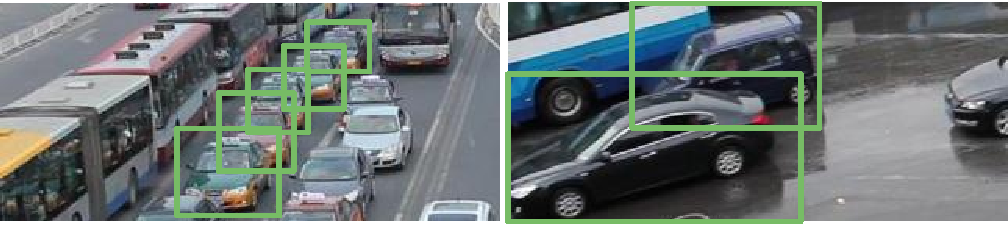
\includegraphics[width=\linewidth]{figures/siamese_tracking/uadetrac_partial_occlusion_multiple_cars.pdf}
    \caption[Partial occlusion in \uadetrac{} dataset]{Partial occlusion in the \uadetrac{} dataset where the object \gls{bbox} covers a great part of the region belonging to another object.}
    \label{fig:UADETRACPartialOcclusionMultiple}
\end{figure}
% ------------------------------------------------------------------------------

Another problem appears during partial occlusion. A vehicle is often severely occluded by another vehicle, so the two \glspl{bbox} enclose both objects (\figtext{}~\ref{fig:UADETRACPartialOcclusionMultiple}). Thus, the embedding distances for the two objects are very close since they become ``polluted''. In terms of the \gls{reid} mechanism, the two delineated regions given by the two \glspl{bbox} of closely positioned objects with severe occlusion are sometimes considered to be the same object. Consequently, the two tracks are merged into one.


% ------------------------------------------------------------------------------
\begin{figure}[!t]
    \centering
    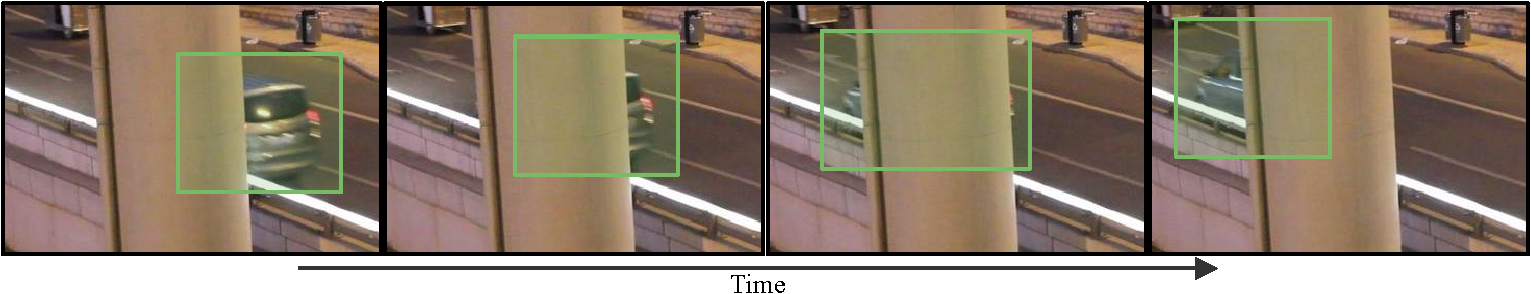
\includegraphics[width=\linewidth]{figures/siamese_tracking/pillar_occlusion.pdf}
    \caption[Pillar occlusion in \uadetrac{} dataset]{A demonstration of almost complete occlusion in the \uadetrac{} dataset where the object passes behind a pillar. As we can see, the tracker correctly infers the object's position based on minor visible cues on the sides of the pillar. However, even if the full occlusion had taken place, thanks to the search region being four times as large as the exemplar region in terms of the area, this object's identity would have been flawlessly recovered, too.}
    \label{fig:UADETRACPillarOcclusion}
\end{figure}
% ------------------------------------------------------------------------------

% ------------------------------------------------------------------------------
\begin{figure}[!t]
    \centering
    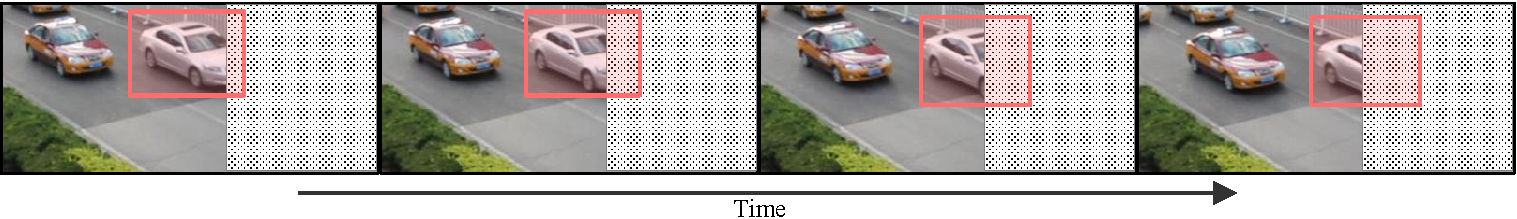
\includegraphics[width=\linewidth]{figures/siamese_tracking/progressing_partial_occlusion.pdf}
    \caption[Progressing occlusion in \uadetrac{} dataset]{Progressing partial occlusion in the \uadetrac{} dataset where a large part of the object \gls{bbox} is covered by a background. In this case, the occlusion comes in a form of a synthetically generated region for demonstration.}
    \label{fig:UADETRACProgressingOcclusion}
\end{figure}
% ------------------------------------------------------------------------------

Besides all this, we did notice that the tracker works well for handling partial occlusion. When the tracked object is only partially occluded, the Siamese tracker properly predicts the possible span of the object (\figtext{}~\ref{fig:UADETRACPillarOcclusion}). This, despite the obvious benefits, posed another challenge to our \gls{reid} extension. We had to store the last visible frame crop for the target object in memory along with its corresponding features for subsequent \gls{reid} in the future. However, the situation depicted in \figtext{}~\ref{fig:UADETRACProgressingOcclusion} shows one of the situations in which the ``last visible exemplar'' was polluted by the occlusion. We would need another mechanism to check for partial occlusion and store only the ``last visible non-occluded exemplar'', or a sequence of multiple exemplars before the visibility confidence dropped below a specific threshold value. The tracker itself maintains a relatively high confidence score anyway, making the whole approach much more complicated.

Thus, to employ \gls{reid} that would utilize the object's most-recent history to re-establish its identity later, there is a need to systematically detect the level of occlusion. With this in mind, the related methods of template updating are worth exploring, too. For instance, Zhang~\etal{}~\cite{zhang2019learning} proposed a replacement for deterministic template updating strategies. They developed a neural network model to learn the optimal template for the next frame while exploiting the current and historical observations of the target object. The template updating based on \gls{gmm} utilized in the \gls{siamrm} tracker together with conditional re-detection could handle long-term object tracking in presence of severe occlusion~\cite{li2019siamrm}. The \gls{gmm} served for dynamically updating the template instead of using a fixed template from the initial frame. But, the template was not updated in every frame or a fixed interval. Instead, only templates with sufficiently high confidence were considered. Even though template updating provides benefits to model adaptation, online tracking may become very inefficient. In addition, it still does not solve the tracking drift problem caused by similar interference completely~\cite{guo2019siamcar}. Moreover, in case of severe occlusion, there is a high risk of the template becoming polluted, which is something we frequently stumbled upon. We dedicated an entire section to various template updating strategies in our survey~\cite{ondrasovic2021siamese}, and we venture to claim that no consensus has been reached so far.

We conjecture that the \gls{reid} is useful for multi-camera scenarios where the task is to re-identify the object from a totally different angle, often without severe occlusion. In common crossroad situations that are abundant in the \uadetrac{} dataset, the first formulation of the online solver approach handles partial occlusion with a lot higher precision than our \gls{reid} extension.

This experiment showed that the inclusion of \gls{reid} mechanism into the inference algorithm brings a lot more disadvantages than benefits and we did not continue with this path. It was not possible to justify the additional complexity we introduced to the model by being able to improve very few cases according to our expectations and by simultaneously exacerbating the performance in other, more frequent situations. Additionally, incorporating this proposal into the tracking pipeline was cumbersome as the underlying design principles had conflicting requirements. For instance, the Siamese tracker head generates predictions even for the dormant tracks. Conversely, we demanded the dormant tracks to become frozen to the last frame where the visibility confidence was satisfactory. This modification was more difficult than we initially expected. There were many other tweaks to the model to make it work, making the whole experiment difficult to conduct.

We think that the architecture in its original formulation is not suited for this type of extension. In fact, we have only observed the integration of \gls{reid} mechanism into the multi-object tracker when the pure tracking-by-detection approach is adopted. After our failure, we are starting to see why. The predictions from the Siamese tracker head have conflicting interests with the \gls{reid} extension. Nonetheless, to address the question of whether a joint training of the tracker and embeddings would bring an improvement, we provide the upcoming experiment, discussed next.
